\documentclass[11pt,class=report,crop=false]{standalone}
\usepackage[screen]{../python}


\begin{document}


%====================================================================
\chapitre{Python : tensorflow avec keras - partie 2}
%====================================================================

\insertvideo{_pC42JErjhk}{partie 10.1. Reconnaissance de chiffres}

\insertvideo{2ZBNRceYWpI}{partie 10.2. Analyse de texte}

\insertvideo{cxxno8F1JmQ}{partie 10.3. Reconnaissance d'images}



\objectifs{Jusqu'ici nous avons travaillé dur pour comprendre en détails la rétropropagation du gradient. Les exemples que nous avons vus reposaient essentiellement sur des réseaux simples. En complément des illustrations mathématiques étudiées, il est temps de découvrir des exemples de la vie courante comme la reconnaissance d'image ou de texte. Nous profitons de la librairie \tensorflow/\keras{} qui en quelques lignes nous permet d'importer des données, de construire un réseau de neurones à plusieurs couches, d'effectuer une descente de gradient et de valider les résultats.}



%%%%%%%%%%%%%%%%%%%%%%%%%%%%%%%%%%%%%%%%%%%%%%%%%%%%%%%%%%%%%%%%%%%%%
\section{Reconnaissance de chiffres}

Il s'agit de reconnaître de façon automatique des chiffres écrits à la main.
\begin{center}
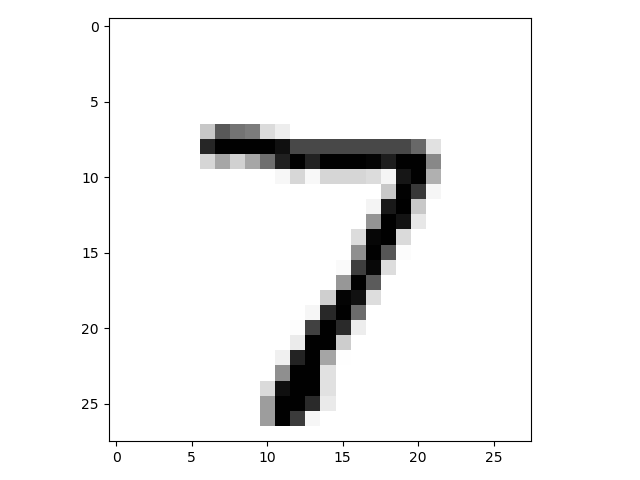
\includegraphics[scale=\myscale,scale=0.20]{figures/tf2-chiffre-test-0}
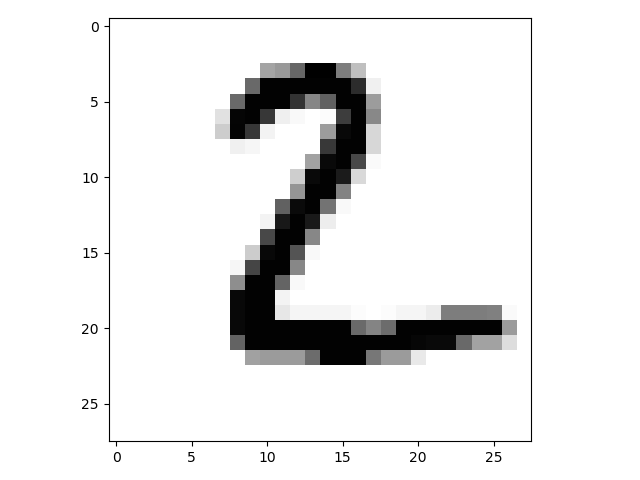
\includegraphics[scale=\myscale,scale=0.20]{figures/tf2-chiffre-test-1}
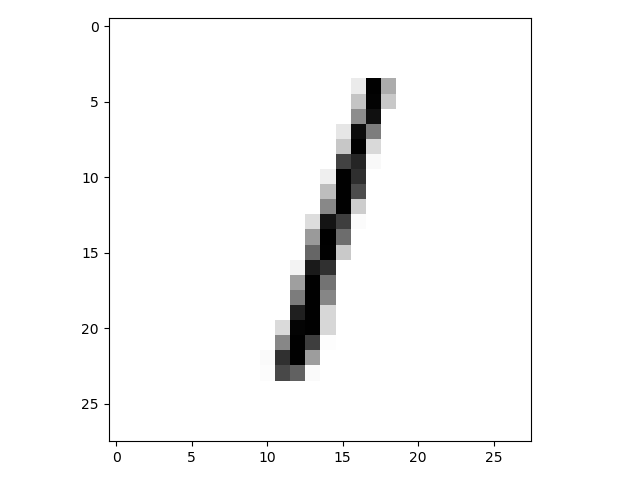
\includegraphics[scale=\myscale,scale=0.20]{figures/tf2-chiffre-test-2}
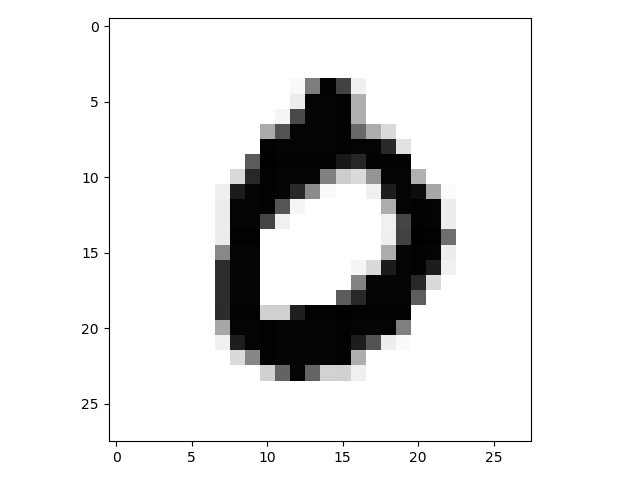
\includegraphics[scale=\myscale,scale=0.20]{figures/tf2-chiffre-test-3}
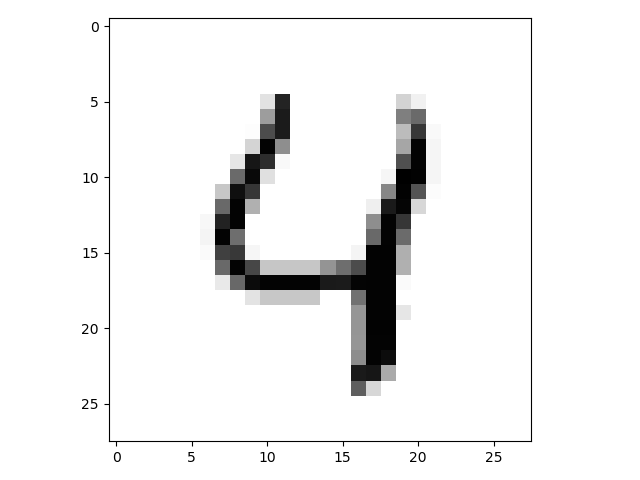
\includegraphics[scale=\myscale,scale=0.20]{figures/tf2-chiffre-test-4}
\end{center}
C'est l'un des succès historiques des réseaux de neurones qui permet par exemple le tri automatique du courrier par lecture du code postal.

%--------------------------------------------------------------------
\subsection{Données}


%---
\subsubsection*{Base MNIST}

\index{donnees@données!MNIST}

Un élément essentiel de l'apprentissage automatique est de disposer de données d'apprentissage nombreuses et de qualité.
Une telle base est la base MNIST dont voici les premières images.
\begin{center}
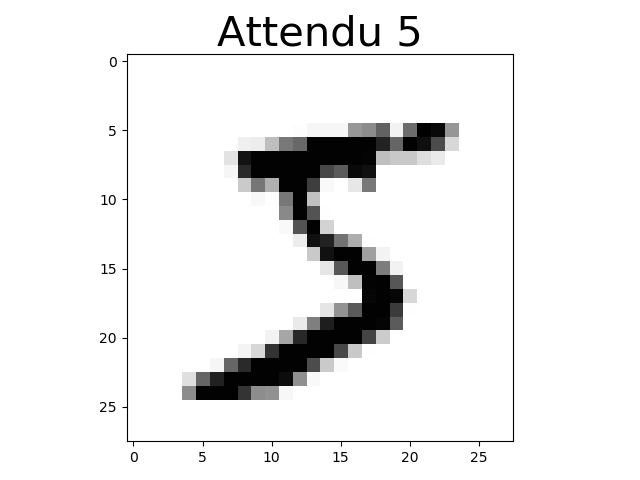
\includegraphics[scale=\myscale,scale=0.20]{figures/tf2-chiffre-train-0}
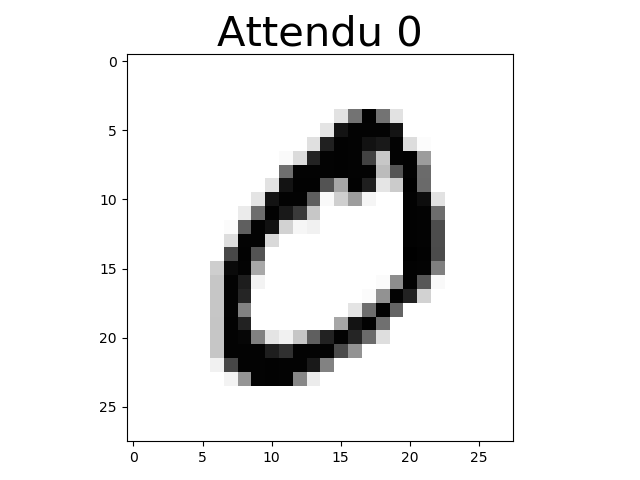
\includegraphics[scale=\myscale,scale=0.20]{figures/tf2-chiffre-train-1}
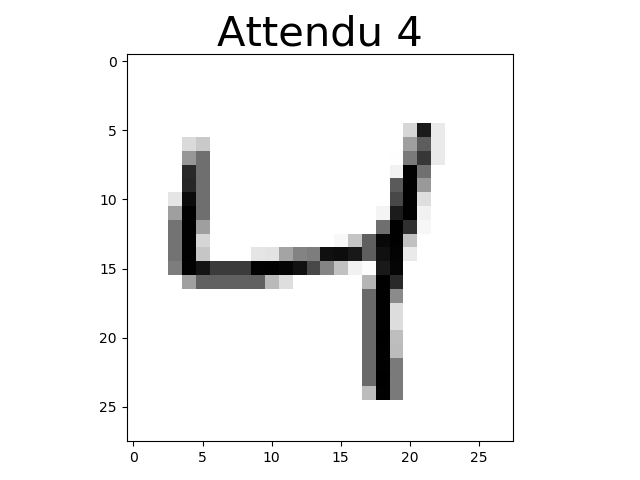
\includegraphics[scale=\myscale,scale=0.20]{figures/tf2-chiffre-train-2}
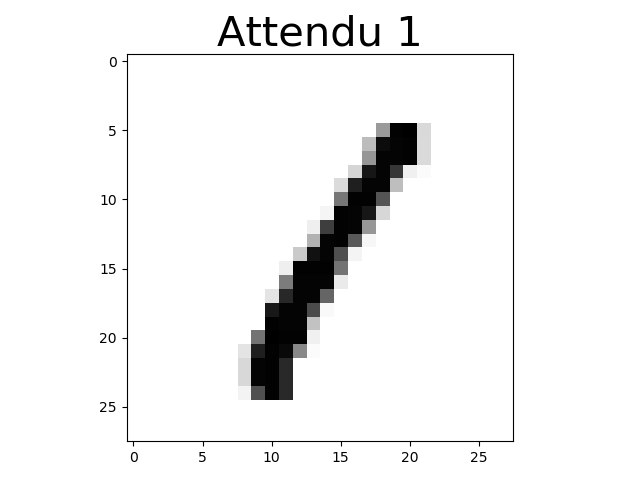
\includegraphics[scale=\myscale,scale=0.20]{figures/tf2-chiffre-train-3}
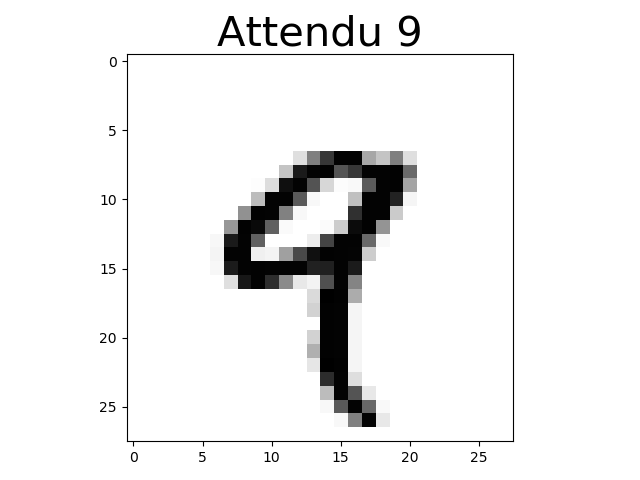
\includegraphics[scale=\myscale,scale=0.20]{figures/tf2-chiffre-train-4}
\end{center}

Une donnée est constituée d'une image et du chiffre attendu.
\begin{center}
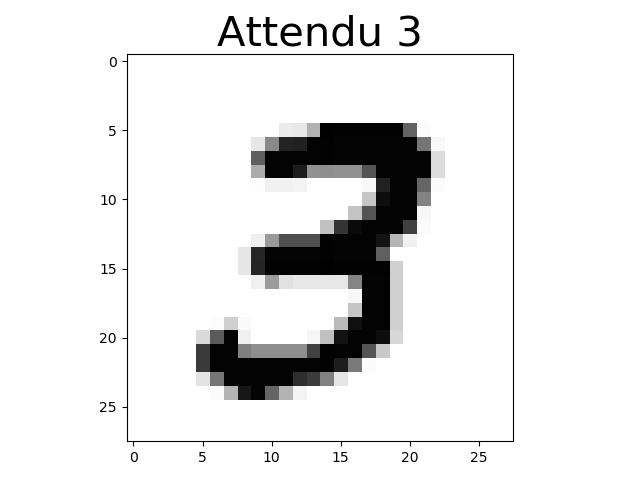
\includegraphics[scale=\myscale,scale=0.5]{figures/tf2-chiffre-train-7}
\end{center}

Plus en détails :
\begin{itemize}
  \item La base est formée de $60\,000$ données d'apprentissage et de $10\,000$ données de test.
  \item Chaque donnée est de la forme : [une image, le chiffre attendu].
  \item Chaque image est de taille $28\times28$ pixels, chaque pixel contenant un des $256$ niveaux de gris (numérotés de $0$ à $255$).
\end{itemize}



Ces données sont accessibles très simplement avec \tensorflow/\keras{} :
\begin{lstlisting}
from tensorflow.keras.datasets import mnist
(X_train_data,Y_train_data),(X_test_data,Y_test_data) = mnist.load_data()
\end{lstlisting} 

Il faut passer un peu de temps à comprendre et à manipuler les données.
\ci{X\_train\_data[i]} correspond à une image et \ci{Y\_train\_data[i]} au chiffre attendu pour cette image. Nous parlerons plus tard des données de test.
On renvoie au fichier \ci{tf2\_chiffres\_data.py} pour une exploration de la base. Noter que l'on peut afficher une image à l'aide de \matplotlib{} par la commande :
\mycenterline{\ci{plt.imshow(X_train_data[i], cmap='Greys')}}
suivie de \ci{plt.show()}.

%---
\subsubsection*{Traitement des données}

Pour une utilisation par un réseau de neurones nous devons d'abord transformer les données.

\bigskip

\textbf{Donnée d'entrée.} En entrée du réseau de neurones, nous devons avoir un vecteur.
Au départ chaque image est un tableau de taille $28\times 28$ ayant des entrées entre $0$ et $255$. Nous la transformons en un vecteur de taille $784 = 28^2$ et nous normalisons les données dans l'intervalle $[0,1]$ (en divisant par $255$). 

\myfigure{0.8}{
  \tikzinput{fig_tf2_06}
}

Ainsi, une entrée $X$ est un \og{}vecteur-image\fg{}, c'est-à-dire un vecteur de taille $784$ représentant une image.

\bigskip

\textbf{Donnée de sortie.} Notre réseau de neurones ne va pas renvoyer le chiffre attendu, mais une liste de $10$ probabilités. Ainsi chaque chiffre doit être codé par une liste de $0$ et de $1$.
\begin{itemize}
  \item $0$ est codé par $(1,0,0,0,0,0,0,0,0,0)$,
  \item $1$ est codé par $(0,1,0,0,0,0,0,0,0,0)$, 
  \item $2$ est codé par $(0,0,1,0,0,0,0,0,0,0)$, 
  \item \ldots
  \item $9$ est codé par $(0,0,0,0,0,0,0,0,0,1)$.
\end{itemize}

\bigskip

\textbf{Fonction.}
Nous cherchons une fonction $F : \Rr^{784} \to \Rr^{10}$, qui à un vecteur-image associe une liste de probabilités, telle que 
$F(X_i) \simeq Y_i$ pour nos données transformées $(X_i,Y_i)$, $i=1,\ldots,60\,000$.

Par exemple la fonction $F$, évaluée sur un vecteur-image $X$ peut renvoyer
$$F(X) = (0.01, 0.04, 0.03, 0.01, 0.02, 0.22, 0.61, 0.02, 0.01, 0.01, 0.02).$$
Dans ce cas, le nombre le plus élevé est $0.61$ au rang $6$, cela signifie que notre fonction $F$ prédit le chiffre $6$ avec une probabilité de $61\%$, mais cela pourrait aussi être le chiffre $5$ qui est prédit à $22\%$. Les autres chiffres sont peu probables.



%---
\subsubsection*{Réseau}

On va construire un réseau de neurones qui produira une fonction $F : \Rr^{784} \to \Rr^{10}$. L'architecture est composée de $3$ couches. En entrée nous avons un vecteur de taille $784$. La première et la seconde couches sont composées chacune de $p=8$ neurones. La couche de sortie est formée de $10$ neurones, un pour chacun des chiffres.


\myfigure{0.8}{
  \tikzinput{fig_tf2_01}
}
%--------------------------------------------------------------------
\subsection{Programme}

Voici le code complet du programme qui sera commenté plus loin.


\begin{lstlisting}
import numpy as np
from tensorflow import keras
from tensorflow.keras import optimizers
from tensorflow.keras.models import Sequential
from tensorflow.keras.layers import Dense

### Partie A - Les données

from tensorflow.keras.datasets import mnist
from tensorflow.keras.utils import to_categorical

# Téléchargement des données
(X_train_data,Y_train_data),(X_test_data,Y_test_data) = mnist.load_data()

N = X_train_data.shape[0]  # N = 60 000 données

# Données d'apprentissage X
X_train = np.reshape(X_train_data,(N,784))  # vecteur image
X_train = X_train/255  # normalisation

# Données d'apprentissage Y vers une liste de taille 10
Y_train = to_categorical(Y_train_data, num_classes=10) 

# Données de test
X_test = np.reshape(X_test_data,(X_test_data.shape[0],784))
X_test = X_test/255
Y_test = to_categorical(Y_test_data, num_classes=10)

### Partie B - Le réseau de neurones

p = 8
modele = Sequential()

# Première couche : p neurones (entrée de dimension 784 = 28x28)
modele.add(Dense(p, input_dim=784, activation='sigmoid'))

# Deuxième couche : p neurones
modele.add(Dense(p, activation='sigmoid'))

# Couche de sortie : 1O neurones (un par chiffre)
modele.add(Dense(10, activation='softmax'))

# Choix de la méthode de descente de gradient
modele.compile(loss='categorical_crossentropy', 
              optimizer='sgd',  
              metrics=['accuracy'])

print(modele.summary())

### Partie C - Calcul des poids par descente de gradient

modele.fit(X_train, Y_train, batch_size=32, epochs=40)

### Partie D - Résultats

resultat = modele.evaluate(X_test, Y_test, verbose=0)
print('Valeur de l''erreur sur les données de test (loss):', resultat[0])
print('Précision sur les données de test (accuracy):', resultat[1])
\end{lstlisting} 


%--------------------------------------------------------------------
\subsection{Résultats}

On estime la performance de notre réseau sur les données de test.
Voici les premiers résultats.

\begin{center}
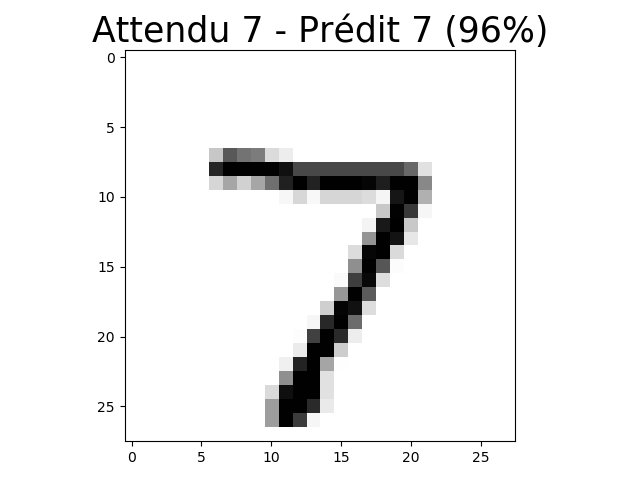
\includegraphics[scale=\myscale,scale=0.20]{figures/tf2-chiffre-test-result-0}
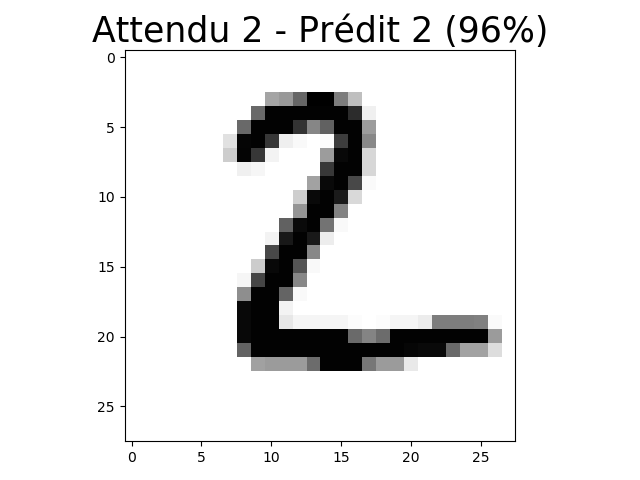
\includegraphics[scale=\myscale,scale=0.20]{figures/tf2-chiffre-test-result-1}
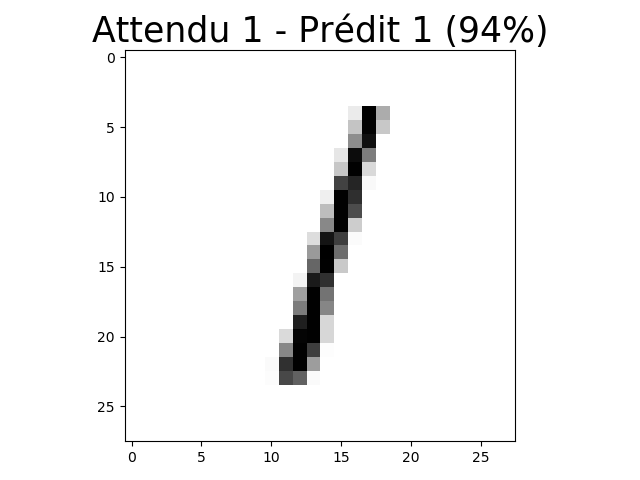
\includegraphics[scale=\myscale,scale=0.20]{figures/tf2-chiffre-test-result-2}
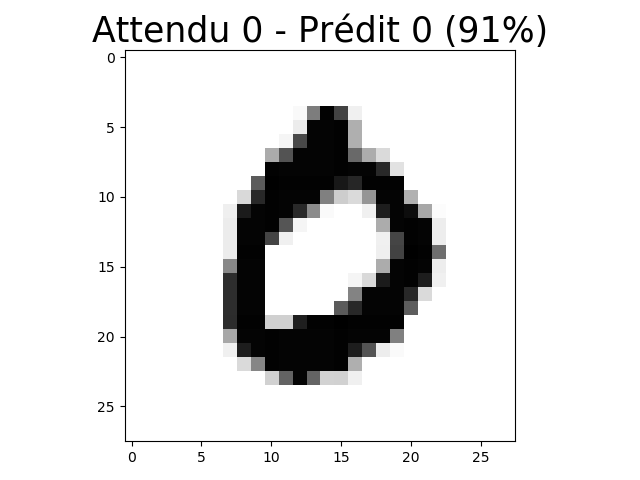
\includegraphics[scale=\myscale,scale=0.20]{figures/tf2-chiffre-test-result-3}
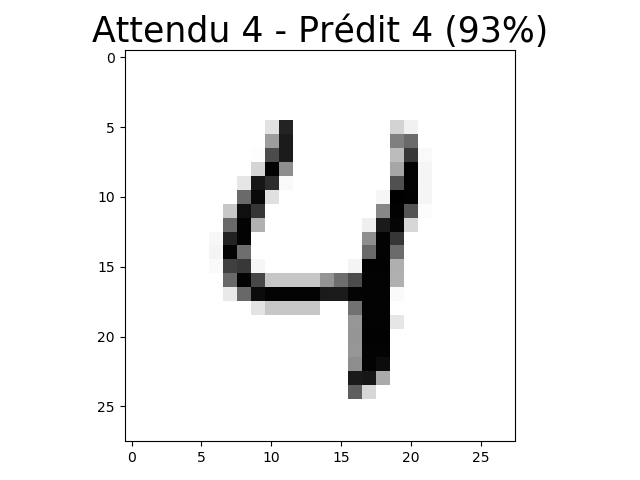
\includegraphics[scale=\myscale,scale=0.20]{figures/tf2-chiffre-test-result-4}
\end{center}
\begin{center}
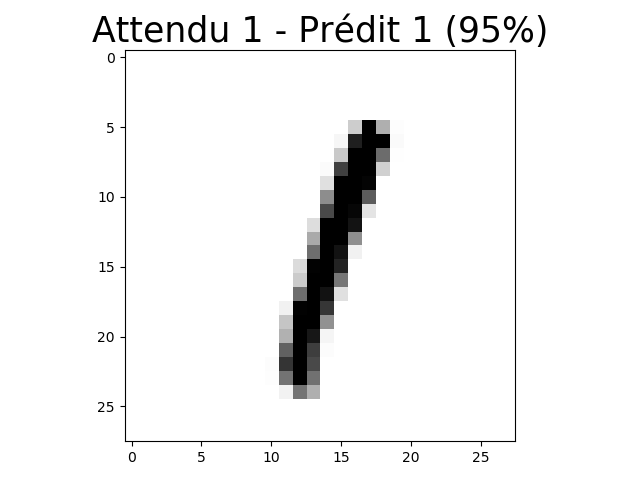
\includegraphics[scale=\myscale,scale=0.20]{figures/tf2-chiffre-test-result-5}
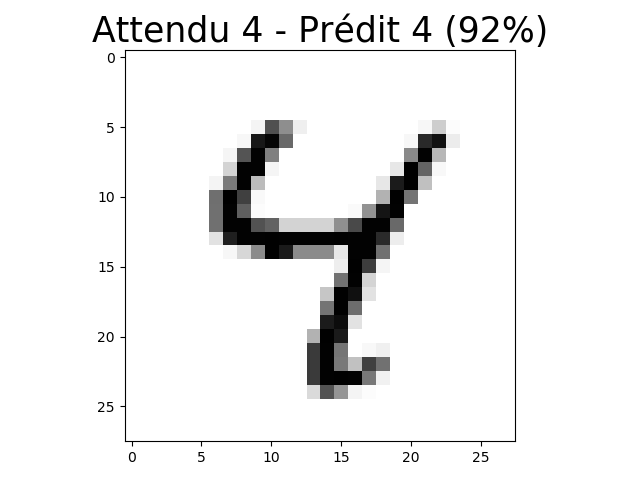
\includegraphics[scale=\myscale,scale=0.20]{figures/tf2-chiffre-test-result-6}
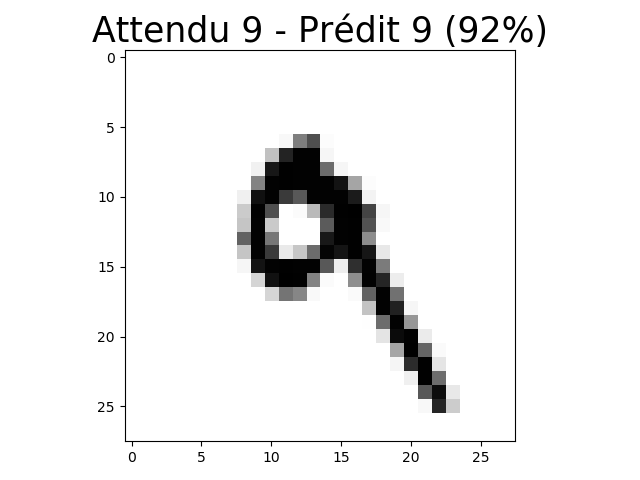
\includegraphics[scale=\myscale,scale=0.20]{figures/tf2-chiffre-test-result-7}
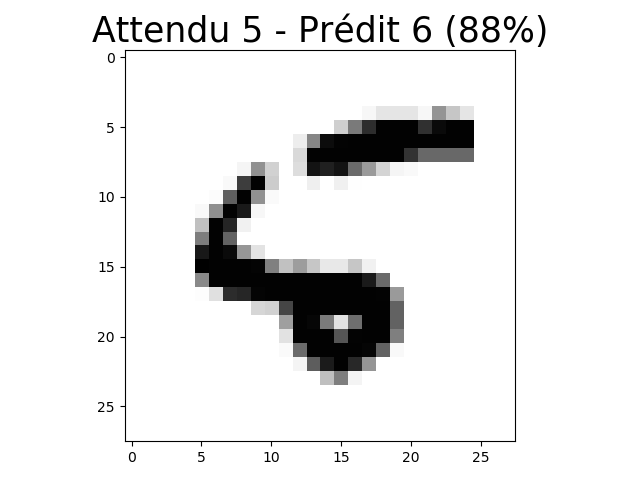
\includegraphics[scale=\myscale,scale=0.20]{figures/tf2-chiffre-test-result-8}
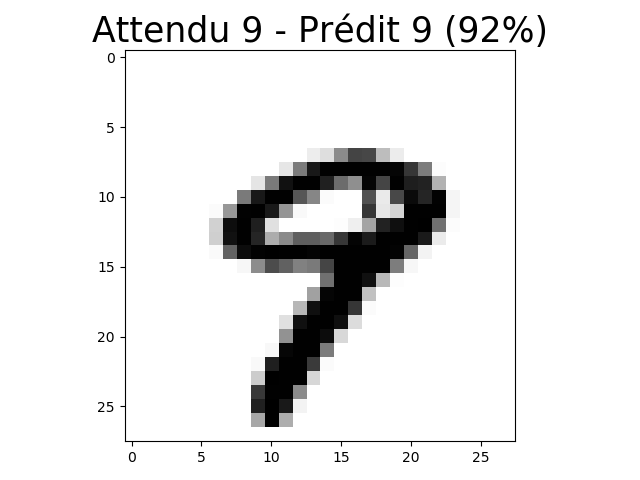
\includegraphics[scale=\myscale,scale=0.20]{figures/tf2-chiffre-test-result-9}
\end{center}

Le réseau prédit correctement $9$ valeurs sur $10$. 
En fait, la fonction associée au réseau renvoie une liste de probabilités. 
Le chiffre prédit est celui qui a la plus forte probabilité.
Par exemple pour la première image (en haut à gauche) la valeur renvoyée est :
$$Y_0 = (0.001, 0.000, 0.000, 0.008, 0.002, 0.005, 0.000, 0.965, 0.000, 0.020).$$
On en déduit la prédiction du chiffre $7$ avec une forte probabilité de $96\%$. 

L'avant-dernière image conduit à une mauvaise prédiction : la fonction prédit le chiffre $6$ alors que le résultat attendu est le chiffre $5$.


Les calculs de la descente de gradient sont faits avec une fonction d'erreur qu'il s'agit de minimiser. Par contre cette fonction d'erreur n'est pas pertinente pour évaluer la qualité de la modélisation. On préfère ici calculer la \defi{précision} (\emph{accuracy}) qui correspond à la proportion de chiffres détectés correctement.

Voici quelques résultats pour différentes tailles du réseau (couche $1$ avec $p$ neurones, couche $2$ avec aussi $p$ neurones, couche $3$ avec $10$ neurones) :
\begin{center}
\begin{tabular}{c|c|c|c}
$p$ & {neurones} & {poids} & {précision} \\ \hline
8 & 26 & 6442 & 90.0\% \\
10 & 30 & 8070 & 91.4\% \\
20 & 50 & 16\,330 & 93.4\% \\
50 & 110 & 42\,310 & 94.4\% \\
\end{tabular}
\end{center}
Sans trop d'efforts on obtient donc une précision de $95\%$. C'est-à-dire que $95$ fois sur $100$ le chiffre prédit est le chiffre correct.

Il est important de mesurer la précision sur les données de test qui sont des données qui n'ont pas été utilisées lors de l'apprentissage. 
Le réseau n'a donc pas appris par c\oe ur les données d'apprentissage, mais a réussi à dégager un schéma, validé sur des données indépendantes.

%--------------------------------------------------------------------
\subsection{Explications}

Reprenons pas à pas le programme et donnons quelques explications.

%---
\subsubsection*{Partie A - Les données}

Les données d'apprentissage sont téléchargées facilement par une seule instruction. Elles regroupent $N=60\,000$ données d'apprentissage (\emph{train}) et $10\,000$ données de test. Les données sont de la forme $(X_i,Y_i)$ où $X_i$ est une image (un tableau $28\times 28$ d'entiers de $0$ à $255$) et $Y_i$ est le chiffre correspondant (de $0$ à $9$).

Les données $X_i$ sont transformées en un  vecteur de taille $784$ (fonction \ci{reshape()}) et ses coefficients sont ramenés dans l'intervalle $[0,1]$ par division par $255$. Ainsi \ci{X\_train} est maintenant une liste \numpy{} de $60\,000$ vecteurs de taille $784$.

Chaque donnée $Y_i$ est transformée en une liste de longueur $10$ du type \ci{[0,0,...,0,1,0,...,0]} avec le $1$ à la place du chiffre attendu. On utilise ici la fonction \ci{to\_categorical()}.



%---
\subsubsection*{Partie B - Le réseau de neurones}

Notre réseau est composé de $3$ couches.
La première couche contient $p=8$ neurones et reçoit en entrée $784$ valeurs (une pour chaque pixel de l'image). La seconde couche contient aussi $p=8$ neurones. La troisième couche contient $10$ neurones (le premier pour détecter le chiffre $0$, le deuxième pour le chiffre $1$,\ldots).
Pour les deux premières couches la fonction d'activation est la fonction $\sigma$. Pour la couche de sortie, la fonction d'activation est la fonction \emph{softmax} qui est adaptée au problème. Ce qui fait que la couche de sortie renvoie une liste de $10$ nombres dont la somme est $1$  et qui correspond à une liste de probabilités.


La fonction d'erreur (\emph{loss}) adaptée au problème s'appelle \ci{categorical\_crossentropy}. La méthode de minimisation de l'erreur choisie est la descente de gradient stochastique.

La valeur \ci{accuracy} du paramètre \ci{metrics} indique que l'on souhaite en plus mesurer la précision des résultats (cela ne change rien pour la descente de gradient qui dépend uniquement de la fonction d'erreur et pas de cette précision).

%---
\subsubsection*{Partie C - Calcul des poids par descente de gradient}

La fonction \ci{fit()}\index{tf@\tensorflow/\keras!fit@\ci{fit()}} lance la descente de gradient (avec une initialisation aléatoire des poids). L'option \ci{batch\_size} détermine la taille du lot (\emph{batch}). On indique aussi le nombre d'époques à effectuer (avec \ci{epochs=40}, chacune des $N = 60\,000$ données sera utilisée $40$ fois, mais comme chaque étape regroupe un lot de $32$ données, il y $40 \times N / 32$ étapes de descente de gradient).



%---
\subsubsection*{Partie D - Résultats}

On insiste sur le fait que la performance du réseau avec les poids calculés doit être mesurée sur les données de test et non sur les données d'apprentissage.

La fonction \ci{evaluate()}\index{tf@\tensorflow/\keras!evaluate@\ci{evaluate()}} renvoie la valeur de la fonction d'erreur (qui est la fonction minimisée par la descente de gradient mais qui n'a pas de signification tangible). Ici la fonction renvoie aussi la précision (car on l'avait demandée en option dans la fonction \ci{compile()}).


%---
\subsubsection*{Un peu plus de résultats}

Pour l'instant, nous avons juste mesuré l'efficacité globale du réseau. Il est intéressant  de vérifier à la main les résultats. Les instructions ci-dessous
calculent les prédictions pour toutes les données de test (première ligne). Ensuite, pour une donnée particulière, on compare le chiffre prédit et le chiffre attendu.


\begin{lstlisting}
# Prédiction sur les données de test
Y_predict = modele.predict(X_test)

# Un exemple
i = 8  # numéro de l'image 

chiffre_predit = np.argmax(Y_predict[i]) # prédiction par le réseau

print("Sortie réseau", Y_predict[i])
print("Chiffre attendu :", Y_test_data[i])
print("Chiffre prédit :", chiffre_predit)

plt.imshow(X_test_data[i], cmap='Greys')  
plt.show()
\end{lstlisting} 

On rappelle que \ci{Y\_predict[i]} est une liste de $10$ nombres correspondant à la probabilité de chaque chiffre. Le chiffre prédit s'obtient en prenant le rang de la probabilité maximale, c'est exactement ce que fait la fonction \ci{argmax} de \numpy{}.



%%%%%%%%%%%%%%%%%%%%%%%%%%%%%%%%%%%%%%%%%%%%%%%%%%%%%%%%%%%%%%%%%%%%%
\section{Fonction d'une variable}


%--------------------------------------------------------------------
\subsection{Données}

Le but est de construire un réseau et de calculer ses poids afin d'approcher la fonction :
$$f(x) = \cos(2x) + x \sin(3x) + \sqrt{x} - 2 \qquad \text{ avec } \  x \in[0,5].$$
\begin{center}
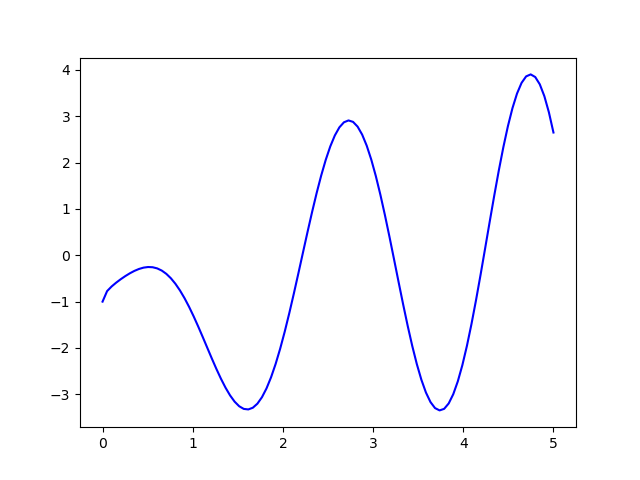
\includegraphics[scale=\myscale,scale=0.5]{figures/unevar-fonction}
\end{center}

On divise l'intervalle de départ $[0,5]$ pour obtenir $N=100$ abscisses $x_i$ qui forment la première partie des données d'apprentissage \ci{X\_train}.
On calcule ensuite les $y_i = f(x_i)$, ce qui donne $100$ ordonnées qui forment l'autre partie des données d'apprentissage \ci{Y\_train}. 


On propose un réseau avec $4$ couches de $10$ neurones, tous de fonction d'activation la fonction tangente hyperbolique, et d'une couche de sortie formée d'un seul neurone de fonction d'activation l'identité.
L'entrée et la sortie sont de dimension $1$. 
La fonction associée au réseau est donc $F : \Rr \to \Rr$.
On souhaite calculer les poids du réseau de sorte que $F(x) \simeq f(x)$, pour tout $x\in[0,5]$.

\myfigure{0.75}{
  \tikzinput{fig_tf2_02}
}

%--------------------------------------------------------------------
\subsection{Programme}

\begin{lstlisting}
# Partie A. Données

# Fonction à approcher
def f(x):
    return np.cos(2*x) + x*np.sin(3*x) + x**0.5 - 2

a, b = 0, 5                 # intervalle [a,b]
N = 100                     # taille des données
X = np.linspace(a, b, N)    # abscisses
Y = f(X)                    # ordonnées
X_train = X.reshape(-1,1)
Y_train = Y.reshape(-1,1)

# Partie B. Réseau 

modele = Sequential()

p = 10
modele.add(Dense(p, input_dim=1, activation='tanh'))
modele.add(Dense(p, activation='tanh'))
modele.add(Dense(p, activation='tanh'))
modele.add(Dense(p, activation='tanh'))
modele.add(Dense(1, activation='linear'))

# Méthode de gradient : descente de gradient classique améliorée
mysgd = optimizers.SGD(lr=0.001, decay=1e-7, momentum=0.9, nesterov=True)
modele.compile(loss='mean_squared_error', optimizer=mysgd)
print(modele.summary())

# Partie C. Apprentissage

history = modele.fit(X_train, Y_train, epochs=4000, batch_size=N)

# Partie D. Visualisation

# Affichage de la fonction et de son approximation
Y_predict = modele.predict(X_train)
plt.plot(X_train, Y_train, color='blue')
plt.plot(X_train, Y_predict,  color='red')
plt.show()

# Affichage de l'erreur au fil des époques
plt.plot(history.history['loss'])
plt.show()
\end{lstlisting}

%--------------------------------------------------------------------
\subsection{Explications}

On a personnalisé la méthode de descente de gradient par la commande 
\mycenterline{\ci{
mysgd = optimizers.SGD(lr=0.001, decay=1e-7, momentum=0.9, nesterov=True)
}}
et on demande à utiliser ces paramètres dans la ligne suivante :
\mycenterline{\ci{
modele.compile(loss='mean_squared_error', optimizer=mysgd)
}}

La fonction d'erreur est ici l'erreur quadratique moyenne.
Notre méthode de gradient débute avec un taux d'apprentissage 
$\delta = 0.001$ (variable \ci{lr} pour \emph{learning rate}).
Ce taux d'apprentissage va diminuer à chaque étape de la descente de gradient selon un paramètre $\alpha = 10^{-7}$ (option \ci{decay}, voir la section 2 du chapitre \og{}Descente de gradient\fg{}).
Enfin, on utilise un moment (\emph{momentum}) et l'accélération de Nesterov (voir la section 4 du chapitre \og{}Descente de gradient\fg{}).


Finalement, on lance le calcul des poids : 
\mycenterline{\ci{
history = modele.fit(X_train, Y_train, epochs=4000, batch_size=N)
}}

Ici on effectue $4000$ époques. La taille de l'échantillon est égale à la taille des données $N$, c'est une descente de gradient classique, il y a donc aussi $4000$ étapes dans la descente de gradient.
La variable \ci{history} contient l'historique des valeurs renvoyées par la fonction \ci{fit()} et permet par exemple d'afficher la valeur de l'erreur au fil des époques.



%--------------------------------------------------------------------
\subsection{Résultats}

Le réseau fournit donc une fonction $F : \Rr \to \Rr$ qui approche correctement la fonction $f$ sur l'intervalle $[0,5]$.
\begin{center}
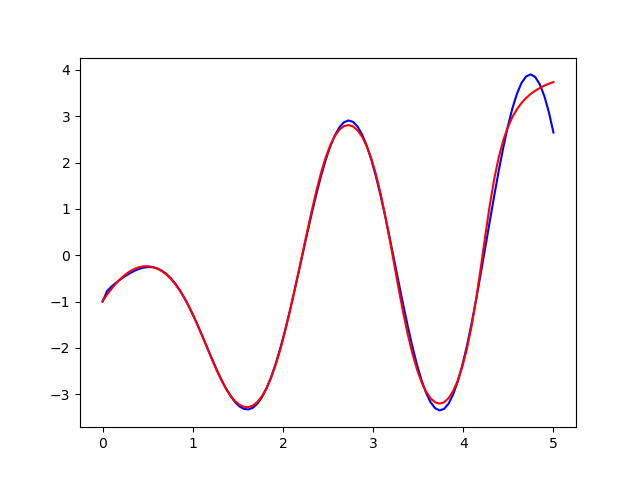
\includegraphics[scale=\myscale,scale=0.5]{figures/unevar-fonction-approx}
\end{center}

Voici le comportement de l'erreur au fil des époques.
\begin{center}
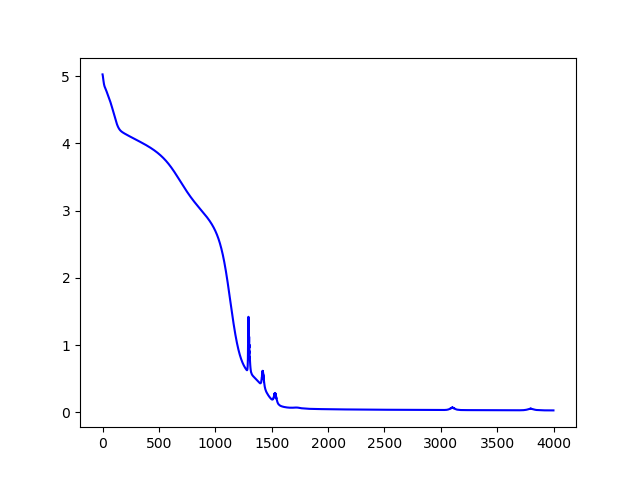
\includegraphics[scale=\myscale,scale=0.5]{figures/unevar-fonction-erreur}
\end{center}

L'erreur n'est pas partout une fonction décroissante, c'est le cas lorsque le taux d'apprentissage est trop grand. D'où l'intérêt de faire diminuer ce taux d'apprentissage au fil des époques à l'aide du paramètre $\alpha$.

Pour terminer, comparons l'évolution des erreurs selon trois méthodes différentes de descente de gradient :
\begin{itemize}
  \item la descente de gradient classique avec $\delta = 0.001$ ;
  \item la descente de gradient classique  améliorée (comme dans le programme ci-dessus) avec $\delta = 0.001$ au départ, mais qui décroît ensuite selon $\alpha = 10^{-7}$, avec un moment et l'accélération de Nesterov ;
  \item la descente de gradient \og{}\emph{adam}\fg{}, qui est une méthode récente et performante, mais plus compliquée que les précédentes.
\end{itemize}

\begin{center}
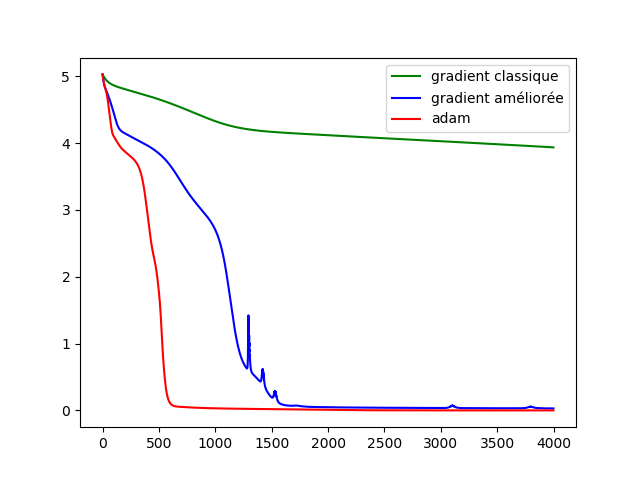
\includegraphics[scale=\myscale,scale=0.5]{figures/unevar-fonction-leserreurs}
\end{center}

On constate des différences importantes de performance. En particulier, pour la méthode classique, il faudrait poursuivre encore longtemps les itérations pour obtenir une erreur raisonnable.


%%%%%%%%%%%%%%%%%%%%%%%%%%%%%%%%%%%%%%%%%%%%%%%%%%%%%%%%%%%%%%%%%%%%%
\section{Quelques fonctionnalités de \tensorflow/\keras}

On revient un peu plus en détails sur l'utilisation de  \tensorflow/\keras.

%--------------------------------------------------------------------
\subsection{Architecture du réseau}

Pour l'instant nous ne travaillons qu'avec un seul type d'architecture de réseaux : des réseaux formés d'une succession de couches de neurones, avec entre deux couches toutes les connexions possibles. On parle de réseaux complètement connectés.

\myfigure{0.8}{
  \tikzinput{fig_tf2_03}
}


Avec \tensorflow/\keras, il suffit de déclarer le modèle du réseau en ajoutant une à une les couches.
\begin{lstlisting} 
modele = Sequential()
modele.add(Dense(N1, input_dim=n, activation='...'))   # première couche
modele.add(Dense(N2, activation='...'))                # deuxième couche
...
modele.add(Dense(p, activation='...'))                 # dernière couche
\end{lstlisting}
La fonction \ci{add()} prend en entrée le nombre $N_i$ de neurones sur cette couche, ainsi que la fonction d'activation des neurones de cette couche.

Pour la première couche (appelée couche d'entrée), il faut également indiquer la dimension des données en entrée par l'option \ci{input_dim=n} où $n$ est la dimension de chaque donnée d'entrée.
Le nombre de neurones $p$ de la dernière couche (appelée couche de sortie) détermine la dimension de chaque donnée de sortie. Ainsi un réseau ayant des entrées de dimension $n$, et $p$ neurones en sortie, détermine une fonction $F : \Rr^n \to \Rr^p$.



%--------------------------------------------------------------------
\subsection{Fonctions d'activation}

\index{fonction d'activation}

\begin{itemize}
  \item \textbf{La fonction ReLU} (pour \emph{Rectified Linear Unit}) s'utilise par l'option \ci{activation='relu'}. Elle est   définie par 
  $$\begin{cases}
  f(x) = 0 & \text{ si } x < 0 \\
  f(x) = x  & \text{ si } x \ge 0 \\
  \end{cases}$$

  \item \textbf{Fonction identité} (option \ci{activation='linear'}) définie par $f(x) = x$. Elle est utile par exemple pour un neurone de sortie.
  
  \item \textbf{La fonction sigmoïde} (option \ci{activation='sigmoid'}) est définie par :
  $$\sigma(x) = \frac{1}{1+e^{-x}}.$$
  Elle prend ses valeurs dans $[0,1]$.
  C'est une version continue de la fonction marche de Heaviside.
    
  \item \textbf{La fonction tangente hyperbolique}
  (option \ci{activation='tanh'}) est définie par :
  $$\tanh(x) = \frac{e^{x}-e^{-x}}{e^{x}+e^{-x}}.$$
  C'est une variante de la fonction sigmoïde qui prend ses valeurs dans $[-1,1]$.
  
\end{itemize}


\begin{minipage}{0.5\textwidth}
\myfigure{0.7}{\tikzinput{fig_activation_relu}}  
\end{minipage}
\begin{minipage}{0.45\textwidth}
\myfigure{0.7}{\tikzinput{fig_activation_linear}}  
\end{minipage}

\begin{minipage}{0.5\textwidth}
\myfigure{0.6}{\tikzinput{fig_activation_sigmoid}}  
\end{minipage}
\begin{minipage}{0.45\textwidth}
\myfigure{0.6}{\tikzinput{fig_activation_tanh}}  
\end{minipage}

%--------------------------------------------------------------------
\subsection{Fonctions d'erreur}

\index{fonction d'erreur}

Pour calculer de bons poids par la descente de gradient, il faut calculer l'erreur entre la sortie attendue et la sortie produite par le réseau. Il faut donc spécifier la méthode utilisée pour calculer cette erreur lorsque l'on finalise le modèle par la commande \ci{compile(loss='...')}.
Plus de détails seront donnés dans le chapitre \og{}Probabilités\fg{}.

Si l'on possède $N$ données d'apprentissage, notons $y_i$ les sorties attendues et $\widetilde y_i$ les sorties produites (calculées par le réseau $\widetilde y_i = F(x_i)$).

\begin{itemize}
  \item \textbf{Erreur quadratique moyenne} (option \ci{loss='mean_squared_error'}). C'est la moyenne des distances au carré :
  $$E = \frac{1}{N} \sum_{i=1}^N (y_i-\widetilde y_i)^2.$$
  Si l'erreur vaut $0$ c'est que toutes les valeurs prédites sont exactement les valeurs attendues.
  
  \item \textbf{Erreur absolue moyenne} (option \ci{loss='mean_absolute_error'}). C'est la moyenne des distances :
  $$E = \frac{1}{N} \sum_{i=1}^N |y_i-\widetilde y_i|.$$
  Intuitivement, cette définition est plus naturelle car elle mesure une distance (et non une distance au carré), mais l'usage de la valeur absolue la rend moins aisée que la précédente.
  
  \item \textbf{Erreur logarithmique moyenne} (option \ci{loss='mean_squared_logarithmic_error'}) qui est :
  $$E = \frac{1}{N} \sum_{i=1}^N \big(\ln(y_i+1) - \ln(\widetilde y_i+1)\big)^2.$$
  L'usage du logarithme est adapté à des données de différentes tailles, car elle prend en compte de façon identique une petite erreur sur une petite valeur et une grande erreur sur une grande valeur.
  
  
  \item \textbf{Entropie croisée binaire} (option \ci{loss='binary_crossentropy'}). Elle est adaptée lorsque le problème a pour sortie attendue $y_i=0$ ou $y_i=1$ et que la sortie produite est une probabilité $\widetilde y_i$ avec $0 \le \widetilde y_i \le 1$.
  
  % $$E = -\frac{1}{N} \sum_{i=1}^N \big( y_i \ln(\widetilde y_i) + (1-y_i) \ln(1-\widetilde y_i)\big).$$
  
  \item \textbf{Entropie croisée pour catégories}  (option \ci{loss='categorical_crossentropy'}). Elle est adaptée lorsque le problème a pour sortie attendue un vecteur du type $y_i=(0,0,\ldots,1,\ldots,0)$ (avec un seul $1$ à la place qui désigne le rang de la catégorie attendue) et la sortie produite est une liste de probabilités $\widetilde y_i = (p_1,p_2,\ldots)$ (voir l'exemple de la reconnaissance de chiffres).
\end{itemize}


%--------------------------------------------------------------------
\subsection{Descente de gradient}

\index{descente de gradient}

Il faut préciser quelle méthode va être utilisée pour minimiser la fonction d'erreur. Cela se fait lors de la finalisation du modèle par la commande \ci{compile(optimizer=...)}. Par contre, la taille de l'échantillon (\emph{batch}) sera précisée plus tard, lors de l'utilisation de la commande \ci{fit()}.

\begin{itemize}
  \item \textbf{Descente de gradient stochastique classique} (option \ci{optimizer='sgd'}). C'est la méthode classique telle qu'elle a été expliquée dans le chapitre \og{}Descente de gradient\fg{}. 
  La taille de l'échantillon permet de faire une descente de gradient stochastique pure 
  (\ci{batch_size=1}), une descente de gradient sur la totalité des $N$ données (\ci{batch_size=N})
  ou toute solution intermédiaire (par exemple \ci{batch_size=32}).

  \item \textbf{Descente de gradient personnalisée améliorée.}
  Par exemple 
  \mycenterline{\ci{
  mysgd = optimizers.SGD(lr=0.001, decay=1e-7, momentum=0.9, nesterov=True)
  }}
  puis un appel par l'option \ci{optimizer=mysgd}.
 
  Les paramètres sont :
  \begin{itemize} 
    \item le taux d'apprentissage $\delta$ (variable \ci{lr}),
    \item le taux $\alpha$ de décroissance de $\delta$ (option \ci{decay}),
    \item le moment (\ci{momentum}),
    \item et l'utilisation ou pas de l'accélération de Nesterov.
  \end{itemize}
  Voir de nouveau le chapitre \og{}Descente de gradient\fg{} pour les détails.
\end{itemize}  
  

Les méthodes de descente sont l'objet de recherches intenses et ont fait d'énormes progrès.
Les nouvelles méthodes sont beaucoup plus performantes et accélèrent grandement les calculs. Mais ces dernières sont trop compliquées et au-delà des objectifs de ce livre, nous n'en donnerons pas d'explications. En voici quelques-unes à tester, parmi celles-ci la méthode \og{}adam\fg{} est l'une des meilleures :
\begin{itemize}
  \item \ci{'adagrad'}
  \item \ci{'adadelta'}
  \item \ci{'rmsprop'}  
  \item \ci{'adam'}  
\end{itemize}  


  

%--------------------------------------------------------------------
\subsection{Mise en place du modèle}

On finalise le modèle par la fonction \ci{compile()}.
\index{tf@\tensorflow/\keras!compile@\ci{compile()}}
\mycenterline{\ci{modele.compile(loss=..., optimizer=...)}}
qui précise le choix de la fonction d'erreur et la méthode de minimisation.
Le réseau est alors initialisé avec des poids aléatoires.

Une fois mis en place, on obtient des informations sur le modèle par la commande:
\mycenterline{\ci{print(modele.summary())}}
qui fournit un résumé chiffré du réseau avec le nombre de couches, le nombre de neurones par couche et le nombre total de poids (coefficients et biais) à calculer. 

On peut vouloir mesurer d'autres choses que la fonction d'erreur.
Par exemple l'option  de la fonction \ci{compile()} : 
\mycenterline{\ci{metrics=['accuracy']}}
va en plus mémoriser la précision du modèle (sous la forme d'un pourcentage de réussite).
Par exemple, si on doit classer des images en deux catégories (chat/$0$ et chien/$1$) alors la fonction d'erreur est un outil indispensable pour notre problème, mais le résultat est mesuré concrètement par le pourcentage d'images correctement identifiées.

Note : pourquoi ne pas prendre la précision comme fonction d'erreur puisque c'est ce qui nous intéresse ? Tout simplement parce que ce n'est pas un fonction différentiable, il n'y a donc pas de méthode de gradient pour la minimiser.


%--------------------------------------------------------------------
\subsection{Calcul des poids}

On lance le calcul des poids par la fonction \ci{fit()} :
\index{tf@\tensorflow/\keras!fit@\ci{fit()}}

\mycenterline{\ci{
modele.fit(X_train, Y_train, batch_size=32, epochs=100)
}}

\begin{itemize}
  \item Les calculs sont effectués selon la méthode de descente de gradient choisie auparavant.
  
  \item Les données d'apprentissage utilisées sont \ci{X\_train} (valeurs de départ) et \ci{Y\_train} (valeurs d'arrivée attendues).
  
  \item L'option \ci{batch_size} précise la taille de l'échantillon:
  \begin{itemize}
      \item une descente de gradient stochastique pure : \ci{batch_size=1},
      \item une descente de gradient sur la totalité des $N$ données : \ci{batch_size=N},
      \item ou toute valeur intermédiaire : par défaut \ci{batch_size=32}.
  \end{itemize}
  
  \item L'option \ci{epochs} détermine le nombre d'étapes dans la méthode de gradient. 
  Si $K$ est la taille d'un lot (valeur de \ci{batch_size}) et $N$ la taille des données alors
  le nombre d'étapes par époque est $N/K$.
  
  \item Il existe une option \ci{verbose} qui permet d'afficher plus ou moins de détails à chaque époque
  ($0$ : rien, $1$ : barre de progression, $2$ : numéro de l'époque).
\end{itemize}

  
%--------------------------------------------------------------------
\subsection{Validation et prédiction}

Une fois les poids calculés, on peut prédire des résultats, c'est-à-dire calculer $F(X)$ pour n'importe quel $X \in \Rr^n$ et pas seulement pour les $X_i$ des données d'apprentissage.
Cela se fait par la fonction \ci{predict()} :
\index{tf@\tensorflow/\keras!predict@\ci{predict()}}
\mycenterline{\ci{
Y_predict = modele.predict(X)
}}

\bigskip

Le calcul des poids par la descente de gradient a pour but de minimiser la fonction d'erreur en utilisant les données d'apprentissage. Mais la pertinence du réseau se mesure sur des données de test qui doivent être indépendantes des données d'apprentissage. La commande

\mycenterline{\ci{
resultat = modele.evaluate(X_test, Y_test)
}}
renvoie la fonction d'erreur calculée sur les données de test (et éventuellement les valeurs demandées par l'option \ci{metrics}).
Si tout va bien, l'erreur sur les données de test devrait être proche de l'erreur sur les données d'apprentissage.




%--------------------------------------------------------------------
\subsection{Poids}


\textbf{Poids.}

La commande \ci{modele.get_weights()}\index{tf@\tensorflow/\keras!get-weights@\ci{get_weights()}} renvoie tous les poids du réseau.
Les poids sont renvoyés sous la forme d'une liste [coefficients de la couche 1, biais de la couche 1, coefficients de la couche 2, \ldots].
On peut aussi travailler couche par couche (voir \og{}Python : tensorflow avec keras - partie 1\fg{}).

\begin{itemize}
  \item Les biais sont donnés sous la forme d'un vecteur (un nombre pour chaque neurone).
  \item Les coefficients sont donnés sous la forme d'un tableau à deux dimensions, dans un ordre contre-intuitif : d'abord les poids de la première entrée pour chaque neurone, puis les poids de la seconde entrée pour chaque neurone, etc.
\end{itemize}

\begin{lstlisting}
poids = [ np.array([[1.,3.,5.], [2.,4.,6.]]),  # Coeff. couche 1
          np.array([-1.,-2.,-3.]),             # Biais couche 1                
          np.array([[7.], [8.], [9.]]),        # Coeff. couche 2
          np.array([-4.]) ]                    # Biais couche 2
\end{lstlisting}

\myfigure{0.7}{\tikzinput{fig_tf2_08}} 

La commande \ci{modele.set_weights(poids)} permet de définir les poids à la valeur voulue.
  
\bigskip
\textbf{Calculs pas à pas.}
La méthode \ci{fit()} effectue un calcul avec un nombre d'époques donné.
On peut travailler étape par étape avec une commande du type :
\mycenterline{\ci{
loss = modele.train_on_batch(X_train, Y_train) 
}}
qui correspond à une étape de descente de gradient.

\bigskip
\textbf{Gradient.}
Il n'est pas facile de récupérer la valeur du gradient avec \tensorflow/\keras.
Le module \ci{keras_facile} propose une fonction \ci{get_weights_grad()} qui renvoie les poids du gradient :
\mycenterline{\ci{
gradient = get_weights_grad(modele, X_train, Y_train)
}}
Les poids du gradient ont la même structure que les poids du réseau.

On peut ainsi programmer facilement à la main sa propre descente de gradient par la commande :
\mycenterline{\ci{
poids_apres = [poids_avant[i] - delta*gradient[i] for i in range(len(poids_avant))]
}}
où \ci{delta} est le taux d'apprentissage (\emph{learning rate}, $\delta=0.1$ par exemple).
Voir le fichier \ci{poids\_gradient.py} pour un exemple.


%%%%%%%%%%%%%%%%%%%%%%%%%%%%%%%%%%%%%%%%%%%%%%%%%%%%%%%%%%%%%%%%%%%%%
\section{Fonction de deux variables}

%--------------------------------------------------------------------
\subsection{Données}
Nous souhaitons construire un réseau pour approcher la fonction de deux variables :
$$f(x,y) = x\cos(y) \text{ avec } \  x \in [-4,4] \text{ et } y \in [-4,4].$$
\begin{center}
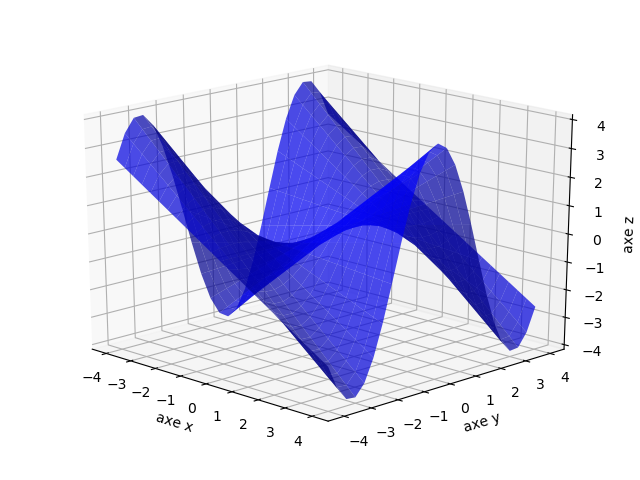
\includegraphics[scale=\myscale,scale=0.5]{figures/tf2-deuxvar-fonction}
\end{center}

On construit un réseau de plusieurs couches, avec deux entrées et une sortie, auquel est donc associée une fonction $F : \Rr^2 \to \Rr$. On souhaite que $F(x,y) \simeq f(x,y)$ 
pour $(x,y) \in [-4,4]^2$. La fonction d'activation est la fonction \og{}ReLU\fg{} (sauf pour le neurone de la couche de sortie qui a pour fonction d'activation l'identité).

\myfigure{0.8}{
  \tikzinput{fig_tf2_04}
}


Les données d'apprentissage sont du type $(x_i,y_i,z_i)$ avec d'une part des $(x_i,y_i)$ sur une grille du carré $[-4,4]^2$ et $z_i = f(x_i,y_i)$.

\myfigure{0.5}{
  \tikzinput{fig_tf2_05}
}

%--------------------------------------------------------------------
\subsection{Programme}

\begin{lstlisting}
# Partie A. Données

# Fonction à approcher
def f(x,y):
    return x*np.cos(y)

n = 25  # pour le nb de points dans la grille
xmin, xmax, ymin, ymax = -4.0, 4.0, -4.0, 4.0

VX = np.linspace(xmin, xmax, n)
VY = np.linspace(ymin, ymax, n)
X, Y = np.meshgrid(VX, VY)
Z = f(X, Y)

entree = np.append(X.reshape(-1,1), Y.reshape(-1,1), axis=1)
sortie = Z.reshape(-1, 1)

# Partie B. Réseau 

modele = Sequential()
p = 10
modele.add(Dense(p, input_dim=2, activation='relu'))
modele.add(Dense(p, activation='relu'))
modele.add(Dense(p, activation='relu'))
modele.add(Dense(1, activation='linear'))

# Méthode de gradient : descente de gradient classique
mysgd = optimizers.SGD(lr=0.01)
modele.compile(loss='mean_squared_error', optimizer=mysgd)
print(modele.summary())

# Partie C. Apprentissage

# Apprentissage époque par époque à la main
for k in range(1000):
    loss = modele.train_on_batch(entree, sortie)
    print('Erreur :',loss)

# Partie D. Visualisation

sortie_produite = modele.predict(entree)
ZZ = sortie_produite.reshape(Z.shape)  # sortie aux bonnes dimensions

# Affichage
import matplotlib.pyplot as plt
from mpl_toolkits.mplot3d import Axes3D

fig = plt.figure()
ax = plt.axes(projection='3d')
ax.plot_surface(X, Y, Z, color='blue', alpha=0.7)
ax.plot_surface(X, Y, ZZ, color='red', alpha=0.7)
plt.show()
\end{lstlisting}

%--------------------------------------------------------------------
\subsection{Explications}

On a ici utilisé la fonctionnalité \ci{train_on_batch()} qui permet d'effectuer une étape de gradient en tenant compte de la totalité des données (cela correspond donc à une époque).


%--------------------------------------------------------------------
\subsection{Résultats}


La fonction prédite est proche de la fonction voulue.

\begin{center}
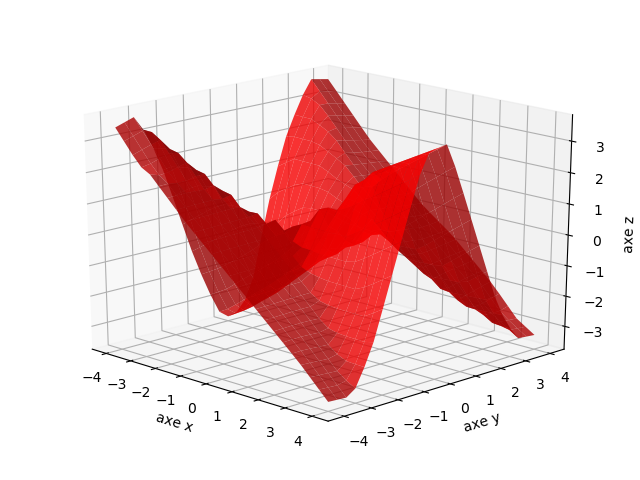
\includegraphics[scale=\myscale,scale=0.5]{figures/tf2-deuxvar-fonction-approx}
\end{center}


%%%%%%%%%%%%%%%%%%%%%%%%%%%%%%%%%%%%%%%%%%%%%%%%%%%%%%%%%%%%%%%%%%%%%
\section{Reconnaissance de texte}

%--------------------------------------------------------------------
\subsection{Données}

Le but de cet exemple est de décider si une critique de film est positive ou négative.
Voici un exemple de critique (la critique numéro $123$) de la base que nous utiliserons :
\begin{quote} 
\emph{beautiful and touching movie rich colors great settings good acting and one of the most charming movies i have seen in a while i never saw such an interesting setting when i was in china my wife liked it so much she asked me to log on and rate it so other would enjoy too}
\end{quote}
C'est un critique positive !


La base IMDB\index{donnees@données!IMDB} fournit $25\,000$ critiques d'apprentissage, chacune étant déjà catégorisée positive (valeur $1$) ou négative (valeur $0$).
Le réseau de neurones pour ce problème va fournir une fonction $F : \Rr^n \to \Rr$.
Si $F(X) \simeq 1$ alors la critique est positive, si $F(X) \simeq 0$ elle est négative.

La première question est : comment transformer le texte d'une critique en un vecteur $X$ de $\Rr^n$ ?
Nous allons l'expliquer sur un exemple simpliste.

Voici trois (fausses) critiques :
\mycenterline{\og{}\emph{bon film à voir absolument}\fg{}\\
\og{}\emph{début moyen mais après c'est très mauvais}\fg{}\\
\og{}\emph{film drôle et émouvant on passe un bon moment}\fg{} \\
}

\begin{itemize}
  \item Tout d'abord, parmi toutes les critiques, on ne retient que les $10$ mots les plus fréquents. Imaginons que ce sont les mots :
\mycenterline{
\emph{film, bon, mauvais, voir, éviter, très, bien, mal, moyen, super}
}
  En réalité on retiendra les $1000$ (voire $10\,000$) mots les plus fréquents.
  
  
  \item On code une phrase comme une liste d'indices de mots.
  Le mot \og{}\emph{film}\fg{} est remplacé par $1$, le mot \og{}\emph{bon}\fg{} par $2$,\ldots{} jusqu'à  \og{}\emph{super}\fg{}. Les autres mots ne sont pas pris en compte.
  Par exemple la critique \og{}\emph{bon film à voir absolument}\fg{} devient la liste d'indices 
  $[2, 1, 4]$. Les deux autres critiques deviennent $[9, 3]$ et $[1, 2]$.
    
  \item On transforme ensuite chaque liste en un vecteur de taille fixe $n=10$ de coordonnées $0$ ou $1$. On place un $1$ en position $i$ si le mot numéro $i$ apparaît dans la critique.
  Ainsi la phrase \og{}\emph{bon film à voir absolument}\fg{}, codée en $[2, 1, 4]$ devient le vecteur
  $X = (1, 1, 0, 1, 0, 0, 0, 0, 0, 0) \in \Rr^{10}$.
  La phrase codée $[9, 3]$ donne le vecteur $X'=(0, 0, 1, 0, 0, 0, 0, 0, 1, 0)$.
  

\myfigure{1}{
  \tikzinput{fig_tf2_09}
}  
   
  \item Ainsi chaque critique est maintenant une entrée $X_i \in \Rr^n$ (avec $n=10$ dans la version simple ci-dessus, mais en réalité ce sera plutôt $n=1000$). Lors de l'apprentissage nous connaissons aussi la sortie attendue $Y_i$ ($0$ ou $1$). On peut alors construire un réseau à $n$ entrées et une seule sortie qui fournit une fonction $F : \Rr^n \to \Rr$ avec pour objectif d'avoir
  $F(X_i) \simeq Y_i$ sur les données d'apprentissage.
  
\end{itemize}

Noter qu'avec ce codage on perd pas mal d'information par rapport à la critique initiale : il manque des mots, l'ordre des mots n'est pas respecté, les mots répétés ne sont pas pris en compte. Mais aussi, \og{}\emph{bon acteur mais mauvais film}\fg{} et \og{}\emph{bon film mais mauvais acteur}\fg{} sont codées par le même vecteur. Malgré cela, on obtient tout de même de très bonnes prédictions !
 
%--------------------------------------------------------------------
\subsection{Programme}

\begin{lstlisting}
# Partie A. Données

from tensorflow.keras.datasets import imdb

# On ne garde que les n=1000 mots les plus fréquents
nb_mots_total = 1000     
(X_train_data, Y_train), (X_test_data, Y_test) = 
                       imdb.load_data(num_words = nb_mots_total)

# Partie A bis. Afficher d'un texte

# Afficher une critique et sa note 
def affiche_texte(num):
    index_mots = imdb.get_word_index()
    index_mots_inverse = dict([(value, key)
                               for (key, value) in index_mots.items()])
    critique_mots = ' '.join([index_mots_inverse.get(i - 3, '??')
                              for i in X_train_data[num]])
    print("Critique :\n", critique_mots)
    print("Note 0 (négatif) ou 1 (positif) ? :", Y_train[num])
    print("Critique (sous forme brute) :\n", X_train_data[num])
    return

affiche_texte(123)   # affichage de la critique numéro 123

# Partie A ter. Données sous forme de vecteurs

def vectorisation_critiques(X_data):
    vecteurs = np.zeros((len(X_data), nb_mots_total))
    for i in range(len(X_data)):
        for c in X_data[i]:
            vecteurs[i,c] = 1.0
    return vecteurs

X_train = vectorisation_critiques(X_train_data)
X_test = vectorisation_critiques(X_test_data)

# Partie B. Réseau 

modele = Sequential()
p = 5
modele.add(Dense(p, input_dim=nb_mots_total, activation='relu'))
modele.add(Dense(p, activation='relu'))
modele.add(Dense(p, activation='relu'))
modele.add(Dense(1, activation='sigmoid'))
modele.compile(loss='binary_crossentropy',
               optimizer='sgd',
               metrics=['accuracy'])

# Partie C. Apprentissage

modele.fit(X_train, Y_train, epochs=10, batch_size=32)


# Partie D. Résultats

Y_predict = modele.predict(X_test)
\end{lstlisting}


%--------------------------------------------------------------------
\subsection{Résultats}

Avec un réseau de seulement $16$ neurones ($5+5+5+1$), la descente de gradient stochastique classique et $10$ époques, nous obtenons une précision entre $80\%$ et $85\%$ sur les données de tests.

Est-ce qu'on peut faire mieux en augmentant le nombre d'étapes ?
Sur le diagramme ci-dessous nous comparons, au fil des époques, la précision obtenue sur les données d'apprentissage avec la précision obtenue sur les données de test.

\begin{center}
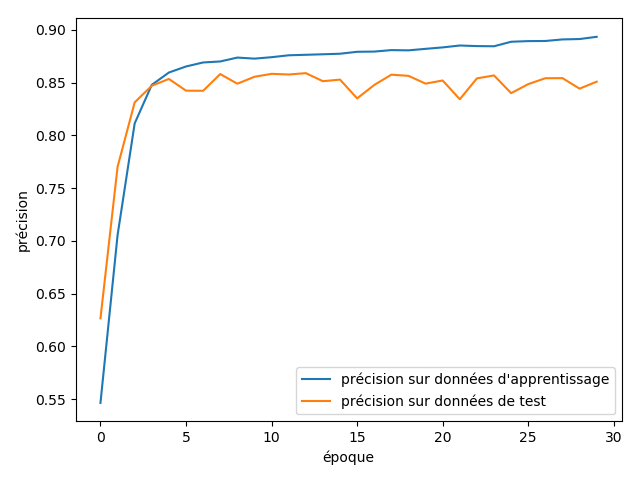
\includegraphics[scale=\myscale,scale=0.5]{figures/tf2-texte-overfit-acc}
\end{center}
La précision calculée sur les données d'apprentissage augmente au fil des époques. Avec un peu plus d'effort, on pourrait même obtenir un précision de $99.9\%$. Par contre, la précision sur les données de test augmente au tout début, puis fluctue autour de $85\%$. 

Que se passe-t-il ? Nous sommes dans une situation de sur-apprentissage ! En augmentant le nombre d'époques, le réseau finit par apprendre par c\oe ur les données d'apprentissage. Par contre, le réseau n'améliore pas les prévisions sur les données de test et n'est donc pas plus performant.

On retrouve ce phénomène sur l'erreur au fil des époques. Elle décroît continuellement vers $0$ sur les données d'apprentissage, alors que sur les données de test, l'erreur ne diminue plus après $5$ époques.

\begin{center}
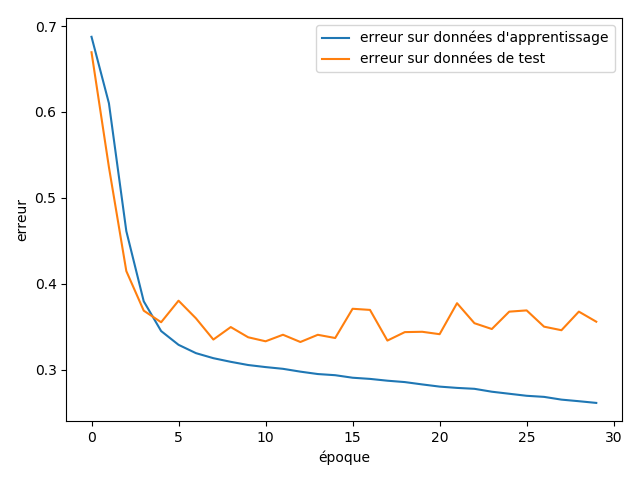
\includegraphics[scale=\myscale,scale=0.5]{figures/tf2-texte-overfit-loss}
\end{center}


%%%%%%%%%%%%%%%%%%%%%%%%%%%%%%%%%%%%%%%%%%%%%%%%%%%%%%%%%%%%%%%%%%%%%
\section{Reconnaissance d'images}

On termine par un constat d'échec (provisoire), nos réseaux de neurones atteignent leurs limites lorsque le problème posé se complique. Nous souhaitons reconnaître des petites images et les classer selon $10$ catégories.

%--------------------------------------------------------------------
\subsection{Données}

La base CIFAR-10\index{donnees@données!CIFAR-10} contient $60\,000$ petites images de $10$ types différents.
\begin{center}
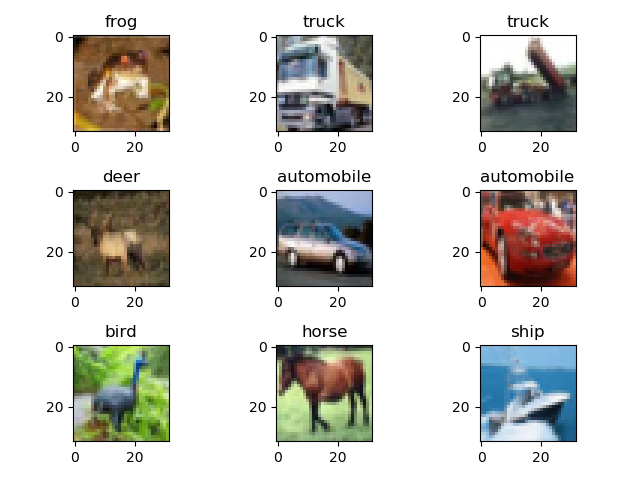
\includegraphics[scale=\myscale,scale=0.7]{figures/tf2-images-train}
\end{center}

Plus en détails :
\begin{itemize}
  \item  Il y a $50\,000$ images pour l'apprentissage et $10\,000$ pour les tests.
  \item Chaque image est de taille $32\times 32$ pixels en couleur. 
  Un pixel couleur est codé par trois entiers $(r,g,b)$ compris entre $0$ et $255$.
  Une image est donc composée de $32\times32\times3$ nombres.
  
  \item Chaque image appartient à une des dix catégories suivantes : avion, auto, oiseau, chat, biche, chien, grenouille, cheval, bateau et camion.
\end{itemize}


%--------------------------------------------------------------------
\subsection{Programme}

\begin{lstlisting}
# Partie A. Données

from tensorflow.keras.datasets import cifar10

(X_train_data,Y_train_data),(X_test_data,Y_test_data)=cifar10.load_data()

num_classes = 10
labels =  ['airplane','automobile','bird','cat','deer',
           'dog','frog','horse','ship','truck']

Y_train = keras.utils.to_categorical(Y_train_data, num_classes)
X_train = X_train_data.reshape(50000,32*32*3)
X_train = X_train.astype('float32')
X_train = X_train/255

# Partie B. Réseau 

modele = Sequential()

p = 30
modele.add(Dense(p, input_dim=32*32*3, activation='sigmoid'))
modele.add(Dense(p, activation='sigmoid'))
modele.add(Dense(p, activation='sigmoid'))
modele.add(Dense(p, activation='sigmoid'))
modele.add(Dense(10, activation='softmax'))

modele.compile(loss='categorical_crossentropy', 
               optimizer='adam', metrics=['accuracy'])

# Partie C. Apprentissage

modele.fit(X_train, Y_train, epochs=10, batch_size=32)
\end{lstlisting}

%--------------------------------------------------------------------
\subsection{Résultats}

Dans le programme ci-dessus avec $p=30$, il y a $100\,000$ poids à calculer.
Avec beaucoup de calculs (par exemple avec $50$ époques et la descente \og{}adam\fg{}), on obtient moins de $50\%$ de précision. Ce qui fait que le sujet d'une image sur deux est mal prédit.


\begin{center}
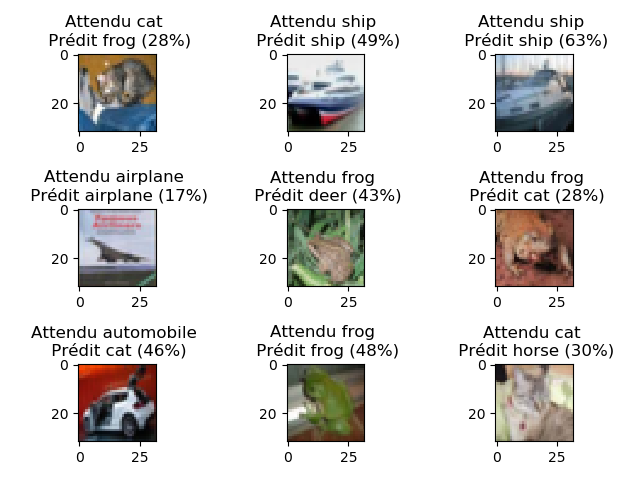
\includegraphics[scale=\myscale,scale=0.7]{figures/tf2-images-test}
\end{center}

Il faut donc une nouvelle approche pour reconnaître correctement ces images !

\end{document}
